\documentclass[11pt,a4paper]{article}
\usepackage[margin=1in,top=0.9in,bottom=0.9in]{geometry}
\usepackage{amsmath,amssymb,booktabs,graphicx,url}
\usepackage[hidelinks]{hyperref}
\newcommand{\RR}{\mathbb R}
\newcommand{\col}{\mathop{\rm col}}
\newcommand{\F}{\mathrm F}
\makeatletter\let\tableinput\@@input\makeatother
\newcommand{\PairCount}{144}
\newcommand{\SmallerCount}{144}
\newcommand{\FullTwo}{6.35}
\newcommand{\MatchTwo}{0.104}
\newcommand{\MatchOne}{6.19}
\newcommand{\SolverGap}{1.06\!\times\!10^{-9}}

\newcommand{\JointPctLo}{2.36}
\newcommand{\JointPctHi}{2.74}
\newcommand{\SepMedianPct}{85.7}
\newcommand{\ExternalPass}{8}
\newcommand{\JointLo}{0.024}
\newcommand{\JointHi}{0.027}
\newcommand{\SepLo}{0.857}
\newcommand{\SepHi}{0.857}
\newcommand{\ExternalInvalid}{0}
\newcommand{\ExternalRefine}{2.4e-10}
\newcommand{\ReviewALo}{0.9970}
\newcommand{\ReviewAHi}{1.0029}
\newcommand{\ReviewBLo}{2.9913}
\newcommand{\ReviewBHi}{2.9977}
\newcommand{\ReviewCalLo}{69.45}
\newcommand{\ReviewCalHi}{69.50}
\newcommand{\ReviewPPMLo}{4.26}
\newcommand{\ReviewPPMHi}{6.15}

\newcommand{\SequentialError}{0.754}
\newcommand{\SequentialCosine}{0.998}
\newcommand{\DirectDiff}{1.91\times10^{-4}}
\newcommand{\RefineDiff}{1.00\times10^{-8}}
\newcommand{\SequentialRatio}{0.247}
\newcommand{\CoupledRatio}{1.003}
\newcommand{\AngleError}{2.26}
\newcommand{\SnapshotSame}{16}
\newcommand{\SnapshotAgreement}{896}
\newcommand{\SnapshotDelta}{3.37e-06}

\title{A two-time-scale law for lagged operator inference on smooth trajectories}
\author{Yunjie Guo \and Hanqing Yang\thanks{Corresponding author. Email:
\href{mailto:hanqing.yang189@gmail.com}{hanqing.yang189@gmail.com}.}}
\date{Independent Researcher, Suzhou, China}
\begin{document}
\maketitle
\begin{abstract}
Lagged features can serve as instruments when fitting an evolution operator to trajectory snapshots. The lag spacing and the forward prediction horizon determine how far this fit moves from ordinary least squares. We derive a finite-sample expansion for the signed change in fitted values when both intervals shrink independently. For $m$ equally spaced lags, a one-step state response with a nonzero projected $m$th derivative gives a change of exact order $h^{2m}$ at spacing $h$, even though the sharp worst-case amplification of the regression residual is of order $h^m$. With two lags and a separate forward horizon $\tau$, the leading scalar is $h^2\tau(\tau+3h)/2$. Omitting the mixed term predicts only one quarter of the leading magnitude at $\tau=h$. We tested the signed matrices against new viscous Burgers and Allen--Cahn trajectory ensembles, sealing numerical predictions before fitting the instruments. An external Lorenz--96 experiment varied the ratio of the two intervals from 0.02 to 50. In the prespecified small-step region, the joint formula had block-median relative errors of \JointPctLo--\JointPctHi\%, compared with approximately \SepMedianPct\% for the separate-limit formula. The block-median fitted changes were only $\ReviewPPMLo$--$\ReviewPPMHi$ parts per million of the state increment in that region. The expansion quantifies estimator agreement on smooth trajectories.
\end{abstract}
\noindent\textbf{Keywords}\quad Operator inference, instrumental variables, principal angles, model reduction, least squares

\section{A discrepancy in a clean-data control}
In discrete-time operator inference, regression maps the present reduced state to the next one using a prescribed feature dictionary \cite{opinf}. With a quadratic dictionary the map is linear in its unknown coefficients. Projecting away spatial degrees of freedom can leave a nonzero regression residual even if every snapshot is exact. Learning models with memory is one response to this loss of information \cite{memory}. We keep the prediction map fixed and ask what happens when earlier values of the dictionary serve as instruments for its current value. Past-snapshot projections also appear in subspace dynamic mode decomposition and noise-resistant approximation of stochastic Koopman operators \cite{takeishi,wanner}. Their statistical goals motivate a finite-sample control. How much can an instrumented fit move even on clean trajectories?

A pilot fit to 100 decaying Burgers trajectories illustrates two different effects. With 20 proper orthogonal decomposition (POD) modes, the two-lag coefficient matrix differed from the full-window ordinary least-squares (OLS) fit by \FullTwo\% in relative Frobenius norm. Refitting OLS on the same current times as the two-lag estimator reduced this difference to \MatchTwo\%. With one lag, the matched difference was \MatchOne\%. Two algebraically equivalent one-lag solvers differed by only $\SolverGap$ in relative coefficient norm. These numbers motivated the study and are reported separately from the independently generated trajectory blocks below.

Three established results locate our contribution. For a regression sketch with orthonormal rows, Chi and Ipsen identified the sharp angular factor controlling the residual contribution to the sketched fit \cite[Prop.~4]{chi}. Taking the sketch to be an orthonormal basis transpose for the instruments gives precisely the factor in Proposition~1 below. Gibson et al.\ related small-window delay coordinates to time derivatives and obtained singular-spectrum scaling laws \cite{gibson}. Koltai and Kunde studied least-squares prediction from a growing set of delay coordinates in an infinite-delay limit \cite{koltai}. Here the number of delays, the current dictionary and the sample rows are fixed. The instrument projector and the target move on separate time scales. We compute their joint effect on the signed difference between fitted maps, including the mixed coefficient and a remainder uniform in the ratio of the intervals (Theorem~4). This coefficient can be tested before either lagged fit is computed.

The missing rows matter in a transient. Write $F$ for all current times, $S$ for those retained after forming lags and $D=F\setminus S$. Let $B_F,B_S$ be the respective OLS fits and $E_D=Y_D-Z_DB_F$. Subtracting the two normal equations gives the grouped deletion identity \cite{cook}
\begin{equation}
 B_S-B_F=-(Z_S^TZ_S)^{-1}Z_D^TE_D. \label{eq:delete}
\end{equation}
The instrumented difference from $B_F$ therefore contains both $B_{\rm IV}-B_S$ and $B_S-B_F$. Their norms need not add. Deleting two starting frames removes two observations \emph{per trajectory}, both at the same physical stage. All subsequent comparisons fix $S$ before changing instruments.

\section{A sharp bound on the common window}
Let $Z\in\RR^{n\times p}$ contain current features, $Y\in\RR^{n\times r}$ the next states, and $W$ the instruments, stacked separately within each trajectory. Let $P$ be the orthogonal projector onto $\col(W)$ and factor $Z=UR$ with $U^TU=I$ and $R$ invertible. Assume $C=U^TPU$ is positive definite. On these rows, $B_0=\arg\min_B\|Y-ZB\|_{\F}$ and $B_W=\arg\min_B\|P(Y-ZB)\|_{\F}$ are unique. The latter is the two-stage least-squares fit. Put $E=Y-ZB_0$, $D_W=Z(B_W-B_0)$ and $s_W=\|D_W\|_{\F}/\|E\|_{\F}$ when $E\ne0$.

\paragraph{Proposition 1 (orthonormal-row sketch bound \cite{chi}).} Let $\theta$ be the largest principal angle from $\col(Z)$ to $\col(W)$. Then
\begin{align}
 D_W &= -U C^{-1} [(I-P)U]^T E, \label{eq:shift}\\
 \sup_{E\ne0,\, U^T E=0} \frac{\|D_W\|_{\F}}{\|E\|_{\F}}
 &=\sqrt{\lambda_{\min}(C)^{-1}-1}=\tan\theta. \label{eq:bound}
\end{align}
For a perfect fit $E=0$, both estimates coincide. Enlarging the instrument space on the same rows weakly decreases this sharp bound. The supremum assumes $n>p$.

\paragraph{Proof.} The projected normal equations give $R(B_W-B_0)=C^{-1}U^TPE$. Since $U^TE=0$, this implies \eqref{eq:shift}. On arbitrary residuals the relevant map in $U$ coordinates is $A=C^{-1}U^TP(I-UU^T)$. Using $P^2=P$ gives $AA^T=C^{-1}-I$. Its largest singular value is attained on a unit residual orthogonal to $U$ whenever the bound is positive. The smallest eigenvalue of $C$ is the square of the smallest singular value of $Q^TU$, for an orthonormal basis $Q$ of $\col(W)$. This singular value is $\cos\theta$, as in classical principal-angle geometry \cite{angles}. For nested spaces the projector difference is positive semidefinite, so the minimum eigenvalue cannot decrease. \hfill\rule{1ex}{1ex}

This ordering applies to a worst case over responses. For example, take $Z=e_1$, $Y=e_3$ in $\RR^3$, and instrument spaces spanned first by $e_1+e_2$, then by $e_1+e_2$ and $e_1+e_3$. The absolute fitted displacement increases from zero to $1/2$, while the bound decreases from $1$ to $1/\sqrt{2}$. The example explains why counting how often actual displacements shrink is an empirical question.


\section{Small-spacing expansion for smooth dictionaries}
Let $Z=[A,F(0)]$ on fixed anchor rows. The columns of $A$ are unchanged by lagging, for example an intercept. Each row of $F(s)$ evaluates the dynamic dictionary on its trajectory at anchor time plus $s$. Take $m$ equally spaced lag blocks and let $P_h$ project onto
\[
 \mathcal W_h=\col[A,F(-h),F(-2h),\ldots,F(-mh)].
\]
In the first expansion the prediction horizon and the response $Y$ are held fixed. Define the derivative space
$\mathcal J=\col[A,F(0),F'(0),\ldots,F^{(m-1)}(0)]$, its orthogonal projector $P_{\mathcal J}$, and
\[
 L=(I-P_{\mathcal J})[0,F^{(m)}(0)]R^{-1}.
\]

\paragraph{Theorem 2.} Suppose that $F$ is $m$ times continuously differentiable near the anchors and the displayed matrix defining $\mathcal J$ has full column rank. As $h\downarrow0$,
\begin{equation}
 \tan\theta_h=h^m\|L\|_2+o(h^m),\qquad
 D_{W_h}=-h^m U L^TE+o(h^m). \label{eq:limit}
\end{equation}
In particular, $L\ne0$ gives exact order $m$ for the worst-case factor. A response with $L^TE=0$ has smaller leading displacement. These statements hold for the fixed sample and coordinate basis, with no distributional assumption on $Y$.

\paragraph{Proof.} Replace the lag blocks by the backward divided differences of orders $0$ through $m-1$ at the same nodes, scaling each by a nonzero constant so its limit is $F^{(j)}(0)$. This invertible block transformation preserves their span for $h>0$. Full rank of the limit implies convergence of the orthogonal projectors to $P_{\mathcal J}$ and hence $C_h=U^TP_hU\to I$. In particular, the projected design has full rank for sufficiently small $h$.

Extrapolating the current features from these $m$ nodes yields
\[
 H_h=\sum_{j=1}^m(-1)^{j+1}\binom{m}{j}F(-jh),
 \qquad F(0)-H_h=h^m F^{(m)}(0)+o(h^m).
\]
This follows entrywise from the backward difference, whose weights cancel all powers below $m$. Since $[A,H_h]$ lies columnwise in $\mathcal W_h$,
\[
 h^{-m}(I-P_h)U
  =(I-P_h)\,[0,h^{-m}(F(0)-H_h)]R^{-1}\ \longrightarrow\ L .
\]
Taking the spectral norm gives the limit of $\sin\theta_h/h^m$. Since $\cos\theta_h\to1$, the first expansion follows. Substituting the matrix limit into \eqref{eq:shift} gives the second. \hfill\rule{1ex}{1ex}

The coefficient depends on the part of the next time derivative that earlier derivatives cannot span, measured after normalizing the current design. There are two ways a displacement can be small. The lagged feature space may almost contain the present one, or the residual may be nearly orthogonal to the remaining direction. The full-column-rank condition on the derivative matrix is sufficient. With redundant derivative columns, extrapolation still gives an $O(h^m)$ upper bound on $\sin\theta_h$ for fixed full-rank $Z$, but the displayed limiting projector requires separate justification. As the POD rank or number of rows changes, $R^{-1}$ and the derivative space change too. The result gives no uniformity over these choices.

\paragraph{Computation.} Use thin QR for $Z$ and an orthonormal basis $Q$ from a rank-revealing decomposition of $W$. Set $M=Q^TU$. Compute the update by solving $\min_X\|MX-Q^TE\|_{\F}$ and then $R(B_W-B_0)=X$. Compute the bound as $\|U-QM\|_2/\sigma_{\min}(M)$. This avoids subtracting two nearly equal fitted operators and forming a cross-product normal matrix. Exact duplicate intercepts can be represented once. Nearly identical lag columns can lose numerical rank as $h$ decreases. In the two-time-scale experiments we also used \eqref{eq:shift} with both factors projected onto the orthogonal complement of the instruments. This replaces the right-hand side by the product of two small defects. That implementation solves with $M^TM$ and cross-checks the displacement with a separate least-squares fit to the increments. In the small-spacing limit $M^TM\to I$. Divided differences offer an equivalent basis in exact arithmetic, but noisy temporal differences can amplify observational error. The raw-feature experiments record numerical rank on every fit.

\paragraph{Manufactured check.} Use the fixed anchors $t_i=-1+i/40$, $i=0,\ldots,80$, a constant and $F(s)_i=(t_i+s)^4$. The derivatives and time shifts are exact polynomials. We evaluated the divided differences from polynomial coefficients and computed $\|L\|_2$ independently from the derivative matrix. Table~\ref{tab:quartic} tests the leading constant. At three lags the two coarsest spacings visibly depart from the limit.
\begin{table}[ht]\centering
\caption{Quartic dictionary. Columns headed by $h$ give $\tan\theta_h/(h^m\|L\|_2)$.}\label{tab:quartic}
\begin{tabular}{rrrrrr}\toprule
$m$ & $\|L\|_2$ & $.050$ & $.020$ & $.010$ & $.005$\\ \midrule
\tableinput quartic.tex
\bottomrule\end{tabular}
\end{table}

\subsection{When the response moves with the instruments}
In a sampled evolution law, shortening the sampling interval often changes two objects at once. The instruments move toward the current features and the response moves toward the current state. Applying the worst-case factor alone then loses an entire power of the interpolation error.

Write $Z(s)=[A,F(s)]$, and suppose that a fixed matrix $S$ selects the state from the dictionary, $q(s)=Z(s)S$. Allow instrument times $-a_1h,\ldots,-a_mh$ for distinct fixed $a_j>0$. The response is $Y_h=q(ch)$ for a fixed $c>0$. Write
\[
 \alpha=\frac{\prod_{j=1}^m a_j}{m!},\qquad
 b(c)=\frac{\prod_{j=1}^m(c+a_j)}{m!},\qquad
 G=(I-P_{\mathcal J})q^{(m)}(0)=LRS .
\]

\paragraph{Theorem 3 (shrinking prediction horizon).}
Under the smoothness and rank conditions of Theorem~2, the change in the fitted state obeys
\begin{equation}
 D_{W_h}=-h^{2m}\alpha\{b(c)-\alpha\}\,U L^T G+o(h^{2m}). \label{eq:coupled}
\end{equation}
If $G\ne0$, this leading matrix is nonzero. For the equally spaced one-step experiment $a_j=j$ and $c=1$, the scalar multiplier is $m$. If also $(I-UU^T)q'(0)\ne0$, the residual-normalized change $s_{W_h}$ has exact order $h^{2m-1}$.

\paragraph{Proof.}
Let $P_h$ project onto the instrument columns. Lagrange extrapolation from the $m$ lag times to $ch$ reproduces polynomials up to degree $m-1$. Its error on the monomial $s^m$ is $h^m\prod_j(c+a_j)$. Taylor expansion on the fixed rows and convergence of the divided-difference spaces therefore give
\begin{align*}
 (I-P_h)U &= h^m\alpha L+o(h^m),\\
 (I-P_h)Y_h &= h^m b(c) G+o(h^m).
\end{align*}
The first line uses extrapolation to the current time and right multiplication by $R^{-1}$. In the second line the extrapolated state columns belong to the instrument space because $q(s)=Z(s)S$. Now let $E_h=(I-UU^T)Y_h$. Since $U^T Y_h\to RS$,
\[
 (I-P_h)E_h=h^m\{b(c)-\alpha\}G+o(h^m).
\]
In \eqref{eq:shift}, $[(I-P_h)U]^T E_h=[(I-P_h)U]^T(I-P_h)E_h$. Multiplying the two leading terms proves \eqref{eq:coupled}. Moreover $(RS)^TL^TG=G^TG$, so $L^TG$ cannot vanish when $G\ne0$. Finally $E_h=ch(I-UU^T)q'(0)+o(h)$, which yields the normalized order. \hfill\rule{1ex}{1ex}

For one lag the typical absolute change is quadratic in $h$. For two it is quartic under the stated nondegeneracy conditions. A bound proportional only to the subspace angle cannot distinguish a distant response from the next state. Equation~\eqref{eq:coupled} explains the extra cancellation through the projection of the response residual. Its coefficient can be computed from the current state and its derivatives before fitting either lagged model. In contrast, the fixed-horizon coefficient in \eqref{eq:limit} also uses the ordinary least-squares residual at the chosen horizon. These are predictions of changes between fitted maps on specified rows. They require separate validation from forecasts of a future trajectory.

\paragraph{A closed vector field.}
The nondegeneracy condition has a concrete consequence in system identification. Take the scalar flow $q'=-q^2$, the dictionary $(q,q^2,1)$ and enough distinct positive anchor states to give full rank and $g=(I-UU^T)q^3\ne0$ (powers act entrywise). With one lag, $G=(I-UU^T)q'=0$, although the quadratic feature has derivative $-2q^3$ and the angular factor has a nonzero linear term. The exact state at horizon $h$ is $q/(1+hq)$. Thus $E_h=h^2 g+O(h^3)$ and \eqref{eq:shift} gives $D_{W_h}=-h^3 U L^T g+o(h^3)$. The leading matrix is nonzero because a column of $LR$ is $-2g$. A quadratic vector field can therefore agree with OLS to cubic order even though the discrete-time flow lies outside the quadratic dictionary. The replication tests evaluate this example and also compare \eqref{eq:coupled} with direct fits for unequal lag spacings and $c=1.75$.

\subsection{Two time scales that approach zero independently}
The preceding result fixes the ratio of the prediction horizon to the lag spacing. In experiments the acquisition interval and the desired forecast horizon are often chosen separately. The following expansion remains informative even if their ratio tends to zero or infinity.

\paragraph{Theorem 4 (uniform two-time-scale expansion).}
Assume the hypotheses of Theorem~3 and $F\in C^{m+1}$ in a neighborhood of the anchors. Write $\tau>0$ for the forward horizon and $\pi_h(s)=\prod_{j=1}^m(s+a_jh)$. As $h,\tau\downarrow0$ independently,
\begin{equation}
 D(h,\tau)=
 -\frac{\alpha h^m}{m!}\{\pi_h(\tau)-\pi_h(0)\}\,U L^TG
 +O\!\left(h^m\tau(h+\tau)^m\right). \label{eq:joint}
\end{equation}
The constants may depend on the finite design, the fixed lag multipliers and derivative bounds. If $G\ne0$, the relative matrix error of the leading prediction is $O(h+\tau)$ uniformly in $\tau/h$.

\paragraph{Proof.}
Set $N_h=I-P_h$ and $V_h=N_h U$. The divided-difference columns of the instruments differ from their limiting derivative columns by $O(h)$. Full rank and smooth dependence of the projector on a full-rank matrix imply $P_h=P_{\mathcal J}+O(h)$. Taylor extrapolation to zero consequently gives $V_h=\alpha h^m L+O(h^{m+1})$. For the response, let $H_h(s)$ be its Lagrange interpolant at the lag nodes. Write the interpolation remainder as
\[
 q(s)-H_h(s)=\pi_h(s)\,d_h(s).
\]
Here $d_h$ is the divided difference of order $m$ at the $m$ lag nodes and $s$. Its simplex integral representation gives $d_h(0)=q^{(m)}(0)/m!+O(h)$ and $\|d_h(\tau)-d_h(0)\|=O(\tau)$, since the next derivative is bounded \cite{deboor}. Every column of $H_h(s)$ belongs to the instrument space. Subtracting at $s=0$ before estimating the two remainders yields
\[
 N_h[q(\tau)-q(0)]
 = \{\pi_h(\tau)-\pi_h(0)\}G/m!+O\!\left(\tau(h+\tau)^m\right).
\]
Indeed $\pi_h(\tau)=O((h+\tau)^m)$ and $\pi_h(\tau)-\pi_h(0)$ is bounded above and below by positive constants times $\tau(h+\tau)^{m-1}$, by positivity of its polynomial coefficients. The OLS residual at $\tau$ is $(I-UU^T)[q(\tau)-q(0)]$. Applying $N_h$ changes the last display by $-V_hU^T[q(\tau)-q(0)]=O(h^m\tau)$. In \eqref{eq:shift}, $C_h^{-1}=I+O(h^{2m})$, since $I-C_h=V_h^TV_h$. Multiplication by $-UC_h^{-1}V_h^T$ proves \eqref{eq:joint}. The lower bound on the polynomial difference and $G^TG=(RS)^TL^TG$ give the relative statement. \hfill\rule{1ex}{1ex}

For consecutive, equally spaced instruments, the scalar multiplying $-UL^TG$ is $h\tau$ for one lag and
\begin{equation}
 \tfrac12 h^2\tau(\tau+3h)\qquad\text{for two lags}. \label{eq:cross}
\end{equation}
Holding $\tau$ fixed in Theorem~2 and then expanding its coefficient for small $\tau$ retains only $h^2\tau^2/2$. At $\tau=h$ this predicts one quarter of the joint leading magnitude; at $\tau\ll h$ the missing term dominates. For a nonzero leading matrix the relative loss from dropping the mixed term is exactly $3h/(\tau+3h)$ at leading order. Keeping this contribution below one quarter therefore requires $\tau>9h$. This is a design rule for the two leading coefficients. At finite spacings each approximation also has a remainder. Both predictions have the same leading direction. This yields a discriminating test on new data: vary the ratio of the two intervals and check the signed matrix relative error, including pairs on either side of $\tau=h$.


\section{Baseline experiments on clean and noisy trajectories}
We generated two families of periodic trajectories on $[0,1)$ for $0\le t\le1$. The viscous Burgers equation $u_t=-u u_x+0.01u_{xx}$ uses 256 spatial points, a Fourier discretization with a two-thirds filter on the nonlinear flux, and exponential time differencing of order four \cite{etd} with step $0.00025$. The Allen--Cahn equation $u_t=0.002u_{xx}+3u(1-u^2)$ uses 128 spatial points and symmetric splitting with step $0.00125$. Its subflows use exact Fourier diffusion and pointwise reaction. A separate refinement test halves the time step and doubles the spatial resolution on three initial conditions, requiring a maximum snapshot-relative error below $10^{-4}$. Both equations start from $0.5\sum_{j=1}^3(g_j/j)\sin(2\pi jx+\phi_j)$ with independent standard-normal $g_j$ and uniform phases.

For each equation we used eight disjoint blocks, each with 40 training and 12 held-out trajectories. Within a block, the training snapshots at times $0,0.005,\ldots,1$ define one uncentered POD basis. Each fit uses its first $r=6,10,16$ modes and a dictionary containing the reduced state, all distinct quadratic monomials, and an intercept. The response is always one sample ahead. Current indices $10,\ldots,199$ give 7,600 training rows at every lag spacing $h=0.005,0.010,0.025$. Past features at $k-h/\Delta t$ define the first space. The second adds features at $k-2h/\Delta t$. The second lag never crosses a trajectory boundary. Held-out trajectories are projected into the training basis. Error norms pool rows and state coordinates within each block.

We fixed this design and primary comparison before examining the new blocks. It was an internal protocol following the pilot. Repeated ranks and spacings within each block share data. The independent experimental units are the eight trajectory ensembles per equation. We report paired ratios, their full range at the shortest spacing, and held-out accuracy. Observations at consecutive times are dependent. No row-level independence assumption enters the calculations.

\paragraph{Use of computational assistance.} OpenAI Codex assisted with the derivations, implementation, execution of the experiments, literature search and drafting. The repository includes the numerical checks, analysis code and block-level summaries used in the manuscript.


\subsection{Agreement between fits and predictive accuracy}
Across both equations, the two-lag fit moved less than the one-lag fit in \SmallerCount{} of \PairCount{} paired evaluations. All projected designs were identifiable at the numerical rank threshold, and all instrument matrices had full column rank. Table~\ref{tab:primary} shows substantial variation in the magnitude of the ratio across ranks and initial-condition ensembles. The displacement uses a prediction norm on the common training rows, so changing units of an individual dictionary column leaves it invariant.
\begin{table}[ht]\centering\small
\caption{Clean trajectories at $h=0.005$. The $s_m$ columns give separate block medians. The last three columns summarize the within-block ratio $s_2/s_1$.}\label{tab:primary}
\begin{tabular}{lrrrrrr}\toprule
Equation & $r$ & $s_1$ & $s_2$ & Median ratio & Min. ratio & Max. ratio\\\midrule
\tableinput paired.tex
\bottomrule\end{tabular}
\end{table}

Figure~\ref{fig:spacing} fixes $r=10$ and varies the physical distance to the instruments while preserving the prediction horizon. Over this grid the one-lag bound follows an approximately linear trend and the two-lag bound rises approximately quadratically. The dotted slopes use the bound at the shortest spacing as their only normalization. The derivative-rank assumption in Theorem~2 holds analytically for the manufactured dictionary. The PDE curves themselves provide a finite-spacing comparison.
\begin{figure}[ht]\centering
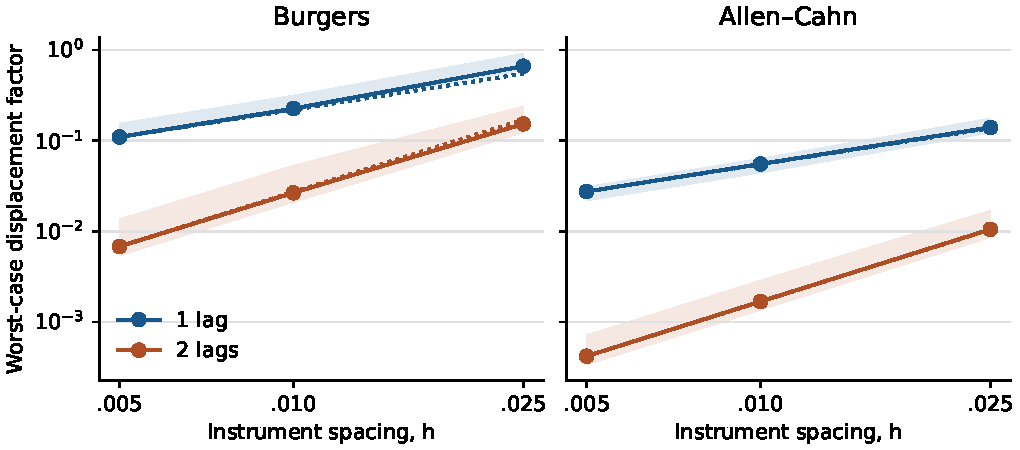
\includegraphics[width=.92\linewidth]{spacing.pdf}
\caption{Sharp displacement factors for the two PDE ensembles at rank 10. Points give block medians, bands span the eight blocks and dotted lines have slopes one and two. All curves use the same anchor times.}\label{fig:spacing}
\end{figure}

\paragraph{Held-out one-step behavior.} For held-out design $Z_*$ and response $Y_*$, the discrepancy between the fitted maps is $g_*=\|Z_*(B_W-B_0)\|_{\F}/\|Y_*\|_{\F}$. A separate quantity $e_*=\|Y_*-Z_*B\|_{\F}/\|Y_*\|_{\F}$ measures predictive error. Table~\ref{tab:test} distinguishes them. A small two-lag displacement preserves most of the OLS error, including any common model misspecification. An improvement count can be positive even if the change is negligible at the precision relevant for prediction.
\begin{table}[ht]\centering\small
\caption{Held-out trajectories at $r=10$, $h=0.005$. Errors and gaps are block medians. Change is the median paired percentage change in error relative to OLS. The count gives blocks with smaller instrumented error.}\label{tab:test}
\begin{tabular}{lrrrrrr}\toprule
Equation & Lags & $g_*$ & OLS $e_*$ & IV $e_*$ & Change (\%) & Count\\\midrule
\tableinput forecast.tex
\bottomrule\end{tabular}
\end{table}

\paragraph{Sensitivity to observation noise.} In a subsequent exploratory check we perturbed all reduced training coordinates by independent Gaussian observations with standard deviation $\rho$ times their pooled clean root-mean-square value. We froze the training basis, used one fixed Gaussian array per block scaled across levels, and fit the same raw quadratic dictionary to noisy inputs and noisy responses. The comparator is OLS on the same noisy rows. At one percent noise, both median paired ratios approach one. The ratio falls again at five percent, so the data give no monotone noise law. Temporal noise disrupts the smooth extrapolation used by Theorem~2. Table~\ref{tab:noise} measures the effect on fit agreement. It cannot identify a noise-corrected physical operator.
\begin{table}[ht]\centering\small
\caption{Noise sensitivity at $r=10$, $h=0.005$. Each group reports median displacements and the median paired ratio.}\label{tab:noise}
\begin{tabular}{rrrrrrr}\toprule
&\multicolumn{3}{c}{Burgers}&\multicolumn{3}{c}{Allen--Cahn}\\
$\rho$ & $s_1$ & $s_2$ & Ratio & $s_1$ & $s_2$ & Ratio\\\midrule
\tableinput noise.tex
\bottomrule\end{tabular}
\end{table}

\section{Predicting the signed displacement before fitting the instruments}
We tested whether the leading matrices in Theorems~2 and~3 predict individual fits at finite spacings. The test used a fresh set of initial conditions, independent of every earlier block. For each equation we drew eight blocks of 32 trajectories. We constructed POD bases from the current states at 37 anchor times $0.05,0.075,\ldots,0.95$, giving 1,184 rows per fit. We used ranks 6 and 10, one and two lags, and seven spacings from $0.00025$ to $0.025$. One arm held the response horizon at $0.005$. The other used the next state at horizon $h$.

At each anchor the semidiscrete right-hand side $f(u)$ and its Jacobian action $f'(u)f(u)$ supplied the first two time derivatives. Each was projected through the fixed POD basis. For a quadratic feature $q_iq_j$ we used $(q_iq_j)''=q_i''q_j+2q_i'q_j'+q_iq_j''$. Neither derivative was estimated from the lagged design. We integrated both semidiscrete equations with fourth-order exponential time differencing, using the original spatial grids and a time step of $0.000125$. A second integration halved the step for block zero of each equation.

\paragraph{Prediction and scoring.}
For each block we stored the signed leading matrices and angular constants, then recorded a SHA-256 digest of the prediction archive before running the scoring stage. The fixed-horizon prediction used the current OLS residual. The coupled prediction used only the current state and its derivatives. To score them, we fit the projected regression on the lagged observations. We computed the difference both by directly fitting state increments and by applying the residual identity in \eqref{eq:shift}. Working in the orthonormal coordinates of $U$ preserves the Frobenius norm and inner product of the fitted changes.

For prediction $\widehat D$ and measured displacement $D$, we scored magnitude and direction jointly with $e=\|\widehat D-D\|_{\F}/\|D\|_{\F}$ and separately recorded the Frobenius cosine. A zero prediction gives $e=1$. Before simulation we defined a usable prediction by $e\le0.25$ and cosine $\ge0.95$, subject to full numerical rank and a displacement above $10^{-13}\|Y-q(0)\|_{\F}$. For each equation, rank, lag count and response arm, the usable range extends from the smallest spacing through the last consecutive grid point with at least seven of eight blocks passing at every point. This definition describes the tested grid. It does not interpolate a continuous cutoff or treat spacings within one block as independent.

\begin{table}[ht]\centering\small
\caption{Maximum spacing in the prespecified usable range. Each entry requires at least seven of eight passing blocks throughout the grid prefix. The final columns give median observed powers $\log_2(\|D(2h)\|/\|D(h)\|)$ at the two smallest spacings with coupled horizon.}\label{tab:ranges}
\begin{tabular}{lrrrrrrr}\toprule
 & & \multicolumn{2}{c}{Fixed horizon} & \multicolumn{2}{c}{Coupled horizon} & \multicolumn{2}{c}{Power}\\
Equation &$r$ & 1 lag & 2 lags & 1 lag & 2 lags & 1 lag & 2 lags\\\midrule
\tableinput ranges.tex
\bottomrule\end{tabular}
\end{table}

At the smallest spacing the predicted coupled displacement had a median relative error below one percent for both lag counts. Its magnitude scaled approximately as $h^2$ and $h^4$, respectively (Table~\ref{tab:ranges}). At the largest spacing the two-lag prediction often missed the tolerance. The fixed-horizon two-lag prediction deteriorated sooner in both equations. With $h=\tau=0.005$ the theoretical one-quarter magnitude ratio predicts a relative error near $0.75$ for the sequential approximation. The fixed-horizon PDE formula uses the measured residual at the chosen horizon. It retains higher powers of the horizon in its coefficient, whereas the separable Lorenz--96 comparator below uses the first Taylor term of that coefficient. The median error of the fixed-horizon PDE formula was $\SequentialError$ and its median cosine was $\SequentialCosine$. On the very same data, the median predicted-to-measured magnitude ratio rose from $\SequentialRatio$ under Theorem~2 to $\CoupledRatio$ under Theorem~3. The median absolute relative error of the angular factor was $\AngleError\%$. Thus the missing response term accounts for a magnitude discrepancy that a check of the angle alone would miss. This comparison motivated the external test of \eqref{eq:cross} below.

\begin{figure}[ht]\centering
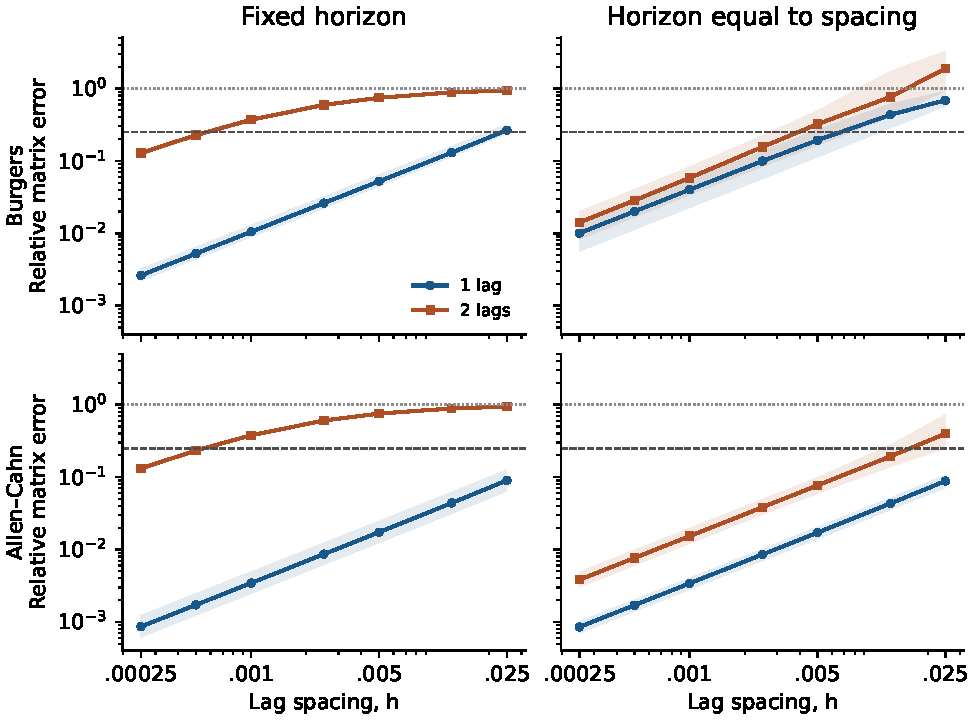
\includegraphics[width=.91\linewidth]{prediction.pdf}
\caption{Prospective relative matrix errors at rank 10. Curves give medians and bands span all eight independent blocks. The dashed line marks the error tolerance of 0.25. The dotted line at one gives the error of predicting zero.}\label{fig:prediction}
\end{figure}

All 896 primary evaluations and 112 integration checks had full numerical rank and resolved displacement. The maximum relative discrepancy between the direct and residualized fit differences was $\DirectDiff$, at a displacement of order $10^{-12}$. Halving the integration step changed the fitted displacement on the common spatial grid by approximately $\RefineDiff$ at its maximum in relative norm across the repeated blocks. The comparison assesses temporal resolution at the specified spatial grid.

\paragraph{A snapshot-only implementation.}
The equation derivatives provide a controlled check. In offline identification, one can instead observe the state at intermediate times. As a separate sensitivity analysis on the same blocks, we acquired three clean forward snapshots per anchor at offsets $\delta,2\delta,3\delta$, with $\delta=0.00075$. These auxiliary times are disjoint from every anchor, lag and response time used for scoring. Writing $d_j=q(j\delta)-q(0)$, we estimated $q'$ by $(18d_1-9d_2+2d_3)/(6\delta)$ and $q''$ by $(-5d_1+4d_2-d_3)/\delta^2$. We used these derivatives in the same formulas with the frozen basis and thresholds. The estimator needs only the four measured states for each derivative calculation. The simulator supplied those additional samples.

Across the 896 predictions the auxiliary-snapshot and equation-based calculations agreed on the pass/fail decision in \SnapshotAgreement{} cases. They gave identical usable grid prefixes in \SnapshotSame{} of the 16 equation, rank, lag-count and horizon combinations. The auxiliary measurements are clean and more frequent than the original training snapshots. Second differentiation scales observation errors by $\delta^{-2}$, so this check does not establish the accuracy of numerical derivatives in the noisy setting of Table~\ref{tab:noise}.

\section{External test of the crossover term}
The two-lag coefficient in \eqref{eq:cross} differs from the product of separate small-spacing and small-horizon factors by the multiplier $1+3h/\tau$. The two formulas predict the same direction, allowing a test of the mixed term using magnitude as well as orientation. After examining the PDE experiment, we fixed this comparison and its decision rule for the 40-variable Lorenz--96 model \cite{lorenz}. No trajectory from this system was used to develop the formulas.

We solved $\dot x_i=(x_{i+1}-x_{i-2})x_{i-1}-x_i+8$ with cyclic indices. Eight independently seeded blocks contained 32 trajectories each. Initial coordinates were $8+N(0,1)$, independently sampled. Classical fourth-order Runge--Kutta integrated five spin-up time units at step $0.005$ and the analyzed segment at step $0.00025$. The block-zero temporal refinement started from the same spin-up endpoints. We reused the anchor schedule and POD ranks of the PDE experiment, then crossed four lag spacings with four forward horizons. The resulting ratios $\tau/h$ range from $0.02$ to $50$. Both the joint and separable forecasts used only the anchor states and their first two time derivatives. A second seal fixed all leading matrices before the first external lag fit.

The primary comparison restricted $h,\tau\le0.005$ and used two lags. For each independent block we first computed its median relative matrix error over the eligible step pairs and both ranks. The criterion required at least seven of eight blocks to give a median of at most $0.25$ for the joint formula and a smaller median than for the separable formula. Table~\ref{tab:external} retains all step pairs.
\begin{table}[ht]\centering\small
\caption{External two-lag prediction on Lorenz--96. Each cell gives the median relative matrix error of the joint and separable formulas (joint / separable) over eight blocks and two ranks. Columns vary the forward horizon, and rows vary lag spacing.}\label{tab:external}
\begin{tabular}{lrrrr}\toprule
$h\backslash\tau$ & 0.00025 & 0.00125 & 0.005 & 0.025\\\midrule
\tableinput crossover_table.tex
\bottomrule\end{tabular}
\end{table}

The primary criterion was met in \ExternalPass{} of eight blocks. Block-median joint errors ranged from \JointPctLo\% to \JointPctHi\%, while the corresponding separable errors clustered around \SepMedianPct\%. At equal steps of $0.005$, the pooled median errors were $0.047$ and $0.749$, respectively. At the largest tested $\tau/h$ the two medians were close, as the mixed term is then small. The eight primary block medians summarize the declared small-step region. The individual cells in Table~\ref{tab:external} additionally reveal where a good region-wide median would conceal a larger local error. Every external grid cell passed the numerical rank and resolution checks. Step refinement on block zero changed the measured displacement by less than $3\times10^{-10}$ in relative norm. This external comparison concerns the fitted displacement. It does not establish improved Lorenz--96 forecasts.

\paragraph{Can a rescaled separable formula explain the improvement?}
After the prespecified test we reanalyzed its 18 primary rank--step combinations per block. Write $T=-h^2\tau^2 U L^TG/2$ for the separable matrix. In each block we estimated $a,b$ by minimizing $\sum_i\|D_i-(a+b h_i/\tau_i)T_i\|_{\F}^2/\|D_i\|_{\F}^2$ over its 18 cells. The theorem predicts $(a,b)=(1,3)$. Across the eight blocks the fitted $a$ ranged from $\ReviewALo$ to $\ReviewAHi$ and $b$ from $\ReviewBLo$ to $\ReviewBHi$. We also set $b=0$, fitted the free scale $a$ on seven blocks using the same loss, and evaluated it on the remaining block. Across the eight held-out blocks this recalibrated formula had median errors of $\ReviewCalLo$--$\ReviewCalHi\%$. The mixed law used its theoretical coefficients throughout. This comparison uses the original external ensembles and is a post hoc sensitivity analysis.

The magnitude of the quantity being predicted sets the numerical significance of these percentages. On the same cells we computed $\|D\|_{\F}/\|q(\tau)-q(0)\|_{\F}$ on the common anchor rows. Its block medians ranged from $\ReviewPPMLo\times10^{-6}$ to $\ReviewPPMHi\times10^{-6}$. Thus in this regime an accurate approximation resolves a small difference between two almost identical fits. The held-out state-prediction errors in Table~\ref{tab:test} address a different performance question.


\section{Interpretation and limits}
When the prediction horizon equals the sampling interval, halving the interval should reduce the clean two-lag fitted change by a factor approaching 16 if $G\ne0$. If the prediction horizon stays fixed, the corresponding factor approaches four when the fixed-response coefficient is nonzero. Choosing between these predictions requires recording both clocks. A lagged-fit comparison can then be made in three steps. First record which current times each method uses and refit the baseline on those times. Next compute the residual-normalized fitted displacement and its angular bound. Finally evaluate both methods on separate trajectories in prediction units. A large coefficient change can accompany a small fitted displacement if the design is poorly conditioned. The factor $R^{-1}$ in the coefficient update makes this sensitivity explicit. Conversely, a nearly unchanged fit can still give poor forecasts if the common dictionary omits important dynamics.

The expansions concern the target of a finite-sample projection on fixed anchor rows. The shrinking-horizon formula additionally assumes that the state is a fixed linear combination of the dictionary columns. The directly computable coefficient uses a full-column-rank derivative matrix. The analytic extension in Section~3 also covers redundant derivatives, using the limiting instrument space. The PDE study uses known right-hand sides to isolate the mathematical effect. With sensor data alone, estimating the derivatives introduces an additional error that this experiment does not quantify. Instrument exogeneity, consistency, deattenuation and long-horizon stability require other evidence. The simulations cover two one-dimensional PDEs and a forced 40-variable model at short lag spacings with clean training bases. They cannot establish a universal preferred lag count or show that the two-lag fit improves noisy-data forecasts. In applications with irregular sampling, rough forcing, measurement noise or near-rank loss, the observed principal angles and held-out errors remain measurable even when the smooth expansion is uninformative.

\section*{Statements and declarations}
\textbf{Funding.} This research received no specific funding.\\
\textbf{Competing interests.} The authors declare no competing interests.\\
\textbf{Data and code availability.} Trajectories are generated from the stated equations and deterministic seed streams. The experiment runners, tests, measured block summaries and manuscript sources are available at \url{https://github.com/fightforbelief/p1-noisy-opinf}.

\begin{thebibliography}{11}
\bibitem{opinf} Peherstorfer, B., Willcox, K.: Data-driven operator inference for nonintrusive projection-based model reduction. Comput. Methods Appl. Mech. Eng. \textbf{306}, 196--215 (2016). \url{https://doi.org/10.1016/j.cma.2016.03.025}
\bibitem{memory} Uy, W.I.T., Peherstorfer, B.: Operator inference of non-Markovian terms for learning reduced models from partially observed state trajectories. J. Sci. Comput. \textbf{88} (2021). \url{https://doi.org/10.1007/s10915-021-01580-2}
\bibitem{takeishi} Takeishi, N., Kawahara, Y., Yairi, T.: Subspace dynamic mode decomposition for stochastic Koopman analysis. Phys. Rev. E \textbf{96}, 033310 (2017). \url{https://doi.org/10.1103/PhysRevE.96.033310}
\bibitem{wanner} Wanner, M., Mezi\'c, I.: Robust approximation of the stochastic Koopman operator. SIAM J. Appl. Dyn. Syst. (2022). \url{https://doi.org/10.1137/21M1414425}
\bibitem{gibson} Gibson, J.F., Farmer, J.D., Casdagli, M., Eubank, S.: An analytic approach to practical state space reconstruction. Physica D \textbf{57}, 1--30 (1992). \url{https://doi.org/10.1016/0167-2789(92)90085-2}
\bibitem{chi} Chi, J.T., Ipsen, I.C.F.: Multiplicative perturbation bounds for multivariate multiple linear regression in Schatten $p$-norms. Linear Algebra Appl. \textbf{624}, 87--102 (2021). \url{https://doi.org/10.1016/j.laa.2021.03.039}
\bibitem{koltai} Koltai, P., Kunde, P.: A Koopman--Takens theorem: linear least squares prediction of nonlinear time series. Commun. Math. Phys. \textbf{405}, 120 (2024). \url{https://doi.org/10.1007/s00220-024-05004-8}
\bibitem{angles} Zhu, P., Knyazev, A.V.: Angles between subspaces and their tangents. J. Numer. Math. \textbf{21}, 325--340 (2013). \url{https://doi.org/10.1515/jnum-2013-0013}
\bibitem{cook} Cook, R.D., Weisberg, S.: Residuals and Influence in Regression. Chapman and Hall, New York (1982).
\bibitem{deboor} de Boor, C.: Divided differences. Surv. Approx. Theory \textbf{1}, 46--69 (2005). \url{https://arxiv.org/abs/math/0502036}
\bibitem{etd} Kassam, A.-K., Trefethen, L.N.: Fourth-order time-stepping for stiff PDEs. SIAM J. Sci. Comput. \textbf{26}, 1214--1233 (2005). \url{https://doi.org/10.1137/S1064827502410633}
\bibitem{lorenz} Lorenz, E.N., Emanuel, K.A.: Optimal sites for supplementary weather observations: simulation with a small model. J. Atmos. Sci. \textbf{55}, 399--414 (1998). \url{https://texmex.mit.edu/ftp/pub/emanuel/PAPERS/lorenz98.pdf}
\end{thebibliography}
\end{document}
